
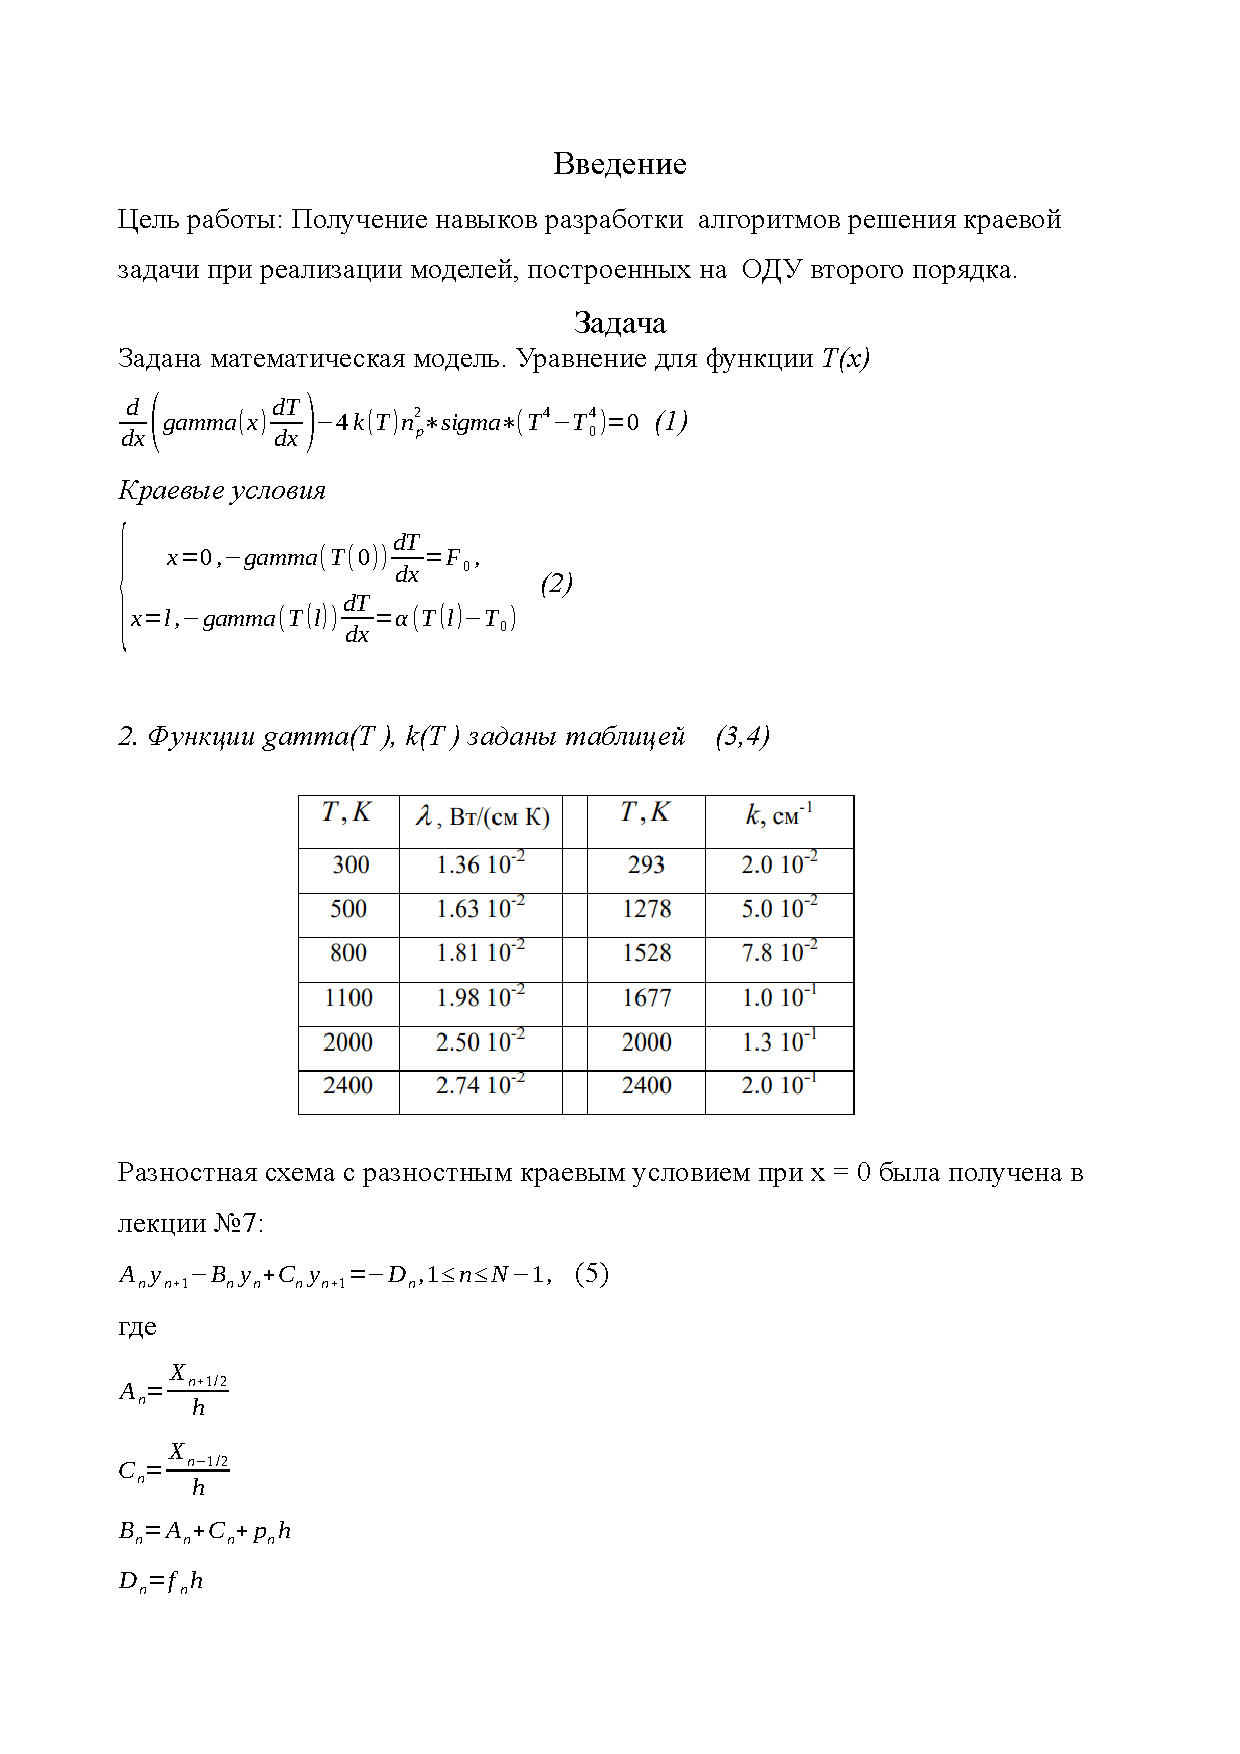
\includepdf[pages=-]{mod_03.pdf}


\section*{Ответы на контрольные вопросы}


\subsection*{1. Какие способы тестирования программы можно предложить?}

Для тестирования можно изменять значение параметра $F_0$:
\begin{itemize}
	\item $F_0 = 0$: отсутствует нагревание, температура стержня по всей его длине должна равняться температуре среды;
	\item $F_0 < 0$: происходить съём тепла, температура должна возрастать до температуры среды.
\end{itemize}

Также можно увеличить коэффициент теплоотдачи в N раз: стержень будет отдавать больше тепла, следовательно, он быстрее будет охлаждаться.


\subsection*{2. Получите простейший разностный аналог нелинейного краевого условия 
$$ x = l, -k(l)\frac{dT}{dx}=\alpha_N(T(l)- T_0) + \varphi(T), $$ где $\varphi(T)$ - заданная функция. Производную аппроксимируйте односторонней разностью.}

\begin{enumerate}
	\item Аппроксимируем производную: $$\frac{dT}{dx} = \frac{y_N - y_{N-1}}{h}$$.
	\item Подставим в исходное уравнение: $$-k(l)\frac{y_N - y_{N-1}}{h}=\alpha_N(y_N - T_0) + \varphi(y_N)$$.
	\item Домножим на $h$, произведём замену $y_{N - 1} = \xi_{N} y_{N} + \eta_{N}$ , получим: 
	$$-k(l)(y_N - \xi_N y_N + \eta_N)=\alpha_N(y_N - T_0)h + \varphi(y_N)h$$.
	\item Получим уравнение относительно $y_N$: $$\varphi(y_N)h + y_N(k_N + \alpha_Nh - k_N \xi_N - k_N \eta_N) - \alpha_NT_0h = 0$$.
\end{enumerate}

\subsection*{3. Опишите алгоритм применения метода прогонки, если при $x = 0$ краевое условие квазилинейное (как в настоящей работе), а при $x = l$, как в п.2.}

\begin{enumerate}
	\item Используя рассчитанные на лекции коэффициенты $M_0, P_0, K_0,$ получим $\xi_1$ и $\eta_1$:
	$$ \xi_1 = -\frac{M_0}{P_0}, \eta_1 = -\frac{K_0}{P_0}.$$ Найдем последующие прогоночные коэффициенты: $$ \xi_{n+1} = \frac{C_n}{B_n - A_n \xi_n}, \eta_{n+1} = \frac{F_n + A_n \eta_n}{B_n - A_n \xi_n}.$$ 
	\item Решив полученное уравнение в п.2, получим значение $y_N$ (решить можно, например, методом дихотомии).
	\item Найдем все неизвестные значения $y_n$ по прогоночной формуле: $$y_n = \xi_{n+1}y_{n+1} + \eta_{n+1} .$$
\end{enumerate}

\subsection*{4. Опишите алгоритм определения единственного значения сеточной функции $y_p$ в одной заданной точке p. Использовать встречную прогонку, т.е. комбинацию правой и левой прогонок (лекция №8). Оба краевых условия линейные. }

\begin{enumerate}
	\item Начальные прогоночные коэффициенты для правой прогонки:
	$$ \xi_1 = -\frac{M_0}{P_0}, \eta_1 = -\frac{K_0}{P_0}.$$
	\item Начальные прогоночные коэффициенты для левой прогонки:
	$$ \alpha_{N-1} = -\frac{M_N}{K_N}, \beta_{N-1} = -\frac{P_N}{K_N }.$$
	\item Прогоночные коэффициенты правой прогонки (от 1 до p-1):
	$$ \xi_{n+1} = \frac{C_n}{B_n - A_n \xi_n}, \eta_{n+1} = \frac{F_n + A_n \eta_n}{B_n - A_n \xi_n} .$$
	\item Прогоночные коэффициенты левой прогонки (от p до N-1):
	$$ \alpha_{n-1} = \frac{A_n}{B_n - C_n \alpha_n}, \beta_{n-1} = \frac{F_n + C_n \beta_n}{B_n - C_n \alpha_n} .$$
	\item Составим систему уравнений из правой и левой прогоночной формулы и выразим $y_p$:
	$$ y_p = \frac{\xi_{n+1} \beta_n + \eta_{n+1}}{1 - \xi_{n+1} \alpha_n} .$$
\end{enumerate}

